% ***************************************************
% Appendix
% ***************************************************
\chapter{Appendix}

Write your appendix here. Following two are examples. 


\section{Neorv32 memory address space layout}
\label{app:mem_address}
\begin{figure}[h!]
    \centering
    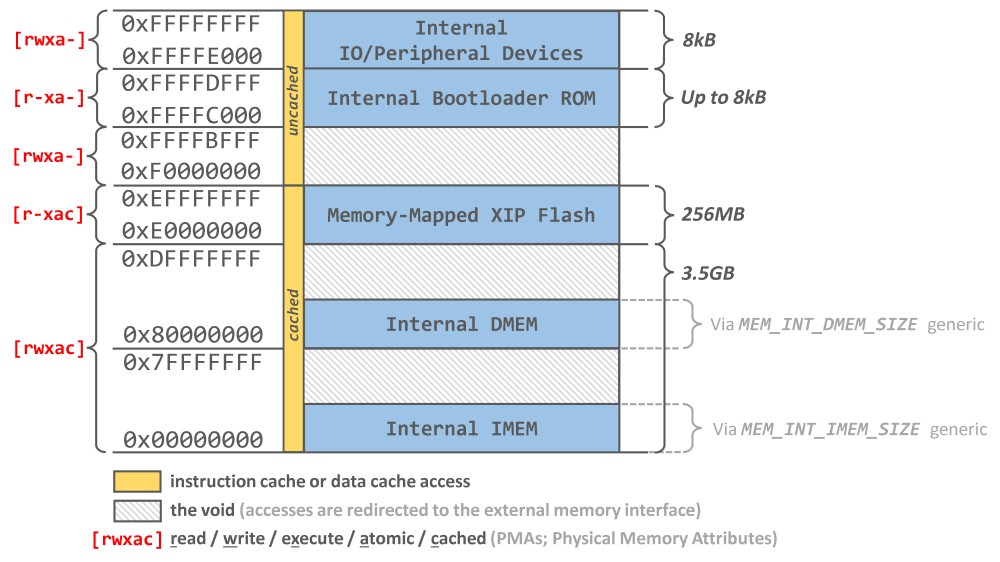
\includegraphics[width=1\textwidth]{Images/neorv32_address_space.png}
    \caption{Neorv32 Memory Address space.}
\end{figure}



\section{FPGA primitives utilisation}
\label{app:res_usage}
\begin{table}
    \centering
    \caption{FPGA primitives utilisation for XC7A100T}
    \begin{tabular}{|l|r|l|}
        \toprule
        Ref Name   & Used & Functional Category \\
        \midrule
        LUT6       & 16262 & LUT \\
        LUT5       & 14820 & LUT \\
        FDRE       & 14500 & Flop \& Latch \\
        LUT3       & 13222 & LUT \\
        MUXF7      &  2436 & MuxFx \\
        FDCE       &  1875 & Flop \& Latch \\
        RAMD64E    &  1836 & Distributed Memory \\
        LUT4       &  1294 & LUT \\
        LUT2       &  1016 & LUT \\
        MUXF8      &   884 & MuxFx \\
        CARRY4     &   437 & CarryLogic \\
        LUT1       &   156 & LUT \\
        RAMB36E1   &   130 & Block Memory \\
        FDPE       &    41 & Flop \& Latch \\
        OBUF       &    40 & IO \\
        LDCE       &    36 & Flop \& Latch \\
        IBUF       &    24 & IO \\
        SRLC32E    &    21 & Distributed Memory \\
        OBUFT      &    11 & IO \\
        BUFG       &     8 & Clock \\
        FDSE       &     5 & Flop \& Latch \\
        DSP48E1    &     4 & Block Arithmetic \\
        SRL16E     &     1 & Distributed Memory \\
        MMCME2\_ADV &    1 & Clock \\
        \bottomrule
    \end{tabular}
\end{table}

\begin{table}
    \centering
    \caption{Memory Utilisation}
    \begin{tabular}{|l|r|r|r|r|r|}
        \toprule
        Site Type      & Used & Fixed & Prohibited & Available & Util\% \\
        \midrule
        Block RAM Tile &  130 &     0 &          0 &       135 & 96.30 \\
        RAMB36/FIFO*   &  130 &     0 &          0 &       135 & 96.30 \\
        RAMB36E1 only  &  130 &     - &          - &         - &    -  \\
        RAMB18         &    0 &     0 &          0 &       270 &  0.00 \\
        \bottomrule
    \end{tabular}
\end{table}

\begin{table}
    \centering
    \caption{Slice Logic Utilisation}
    \begin{tabular}{|l|r|r|r|r|r|}
        \toprule
        Site Type                 & Used & Fixed & Prohibited & Available & Util\% \\
        \midrule
        Slice LUTs*               & 40920 &     0 &          0 &     63400 & 64.54 \\
        LUT as Logic              & 39062 &     0 &          0 &     63400 & 61.61 \\
        LUT as Memory             &  1858 &     0 &          0 &     19000 &  9.78 \\
        LUT as Distributed RAM    &  1836 &     - &          - &         - &    -  \\
        LUT as Shift Register     &    22 &     - &          - &         - &    -  \\
        Slice Registers           & 16457 &     0 &          0 &    126800 & 12.98 \\
        Register as Flip Flop     & 16421 &     0 &          0 &    126800 & 12.95 \\
        Register as Latch         &    36 &     0 &          0 &    126800 &  0.03 \\
        F7 Muxes                  &  2436 &     0 &          0 &     31700 &  7.68 \\
        F8 Muxes                  &   884 &     0 &          0 &     15850 &  5.58 \\
        \bottomrule
    \end{tabular}
\end{table}


\section{Additional webpages built into the webserver.}
\label{app:additional_webpages}
\begin{figure}[h!]
    \centering
    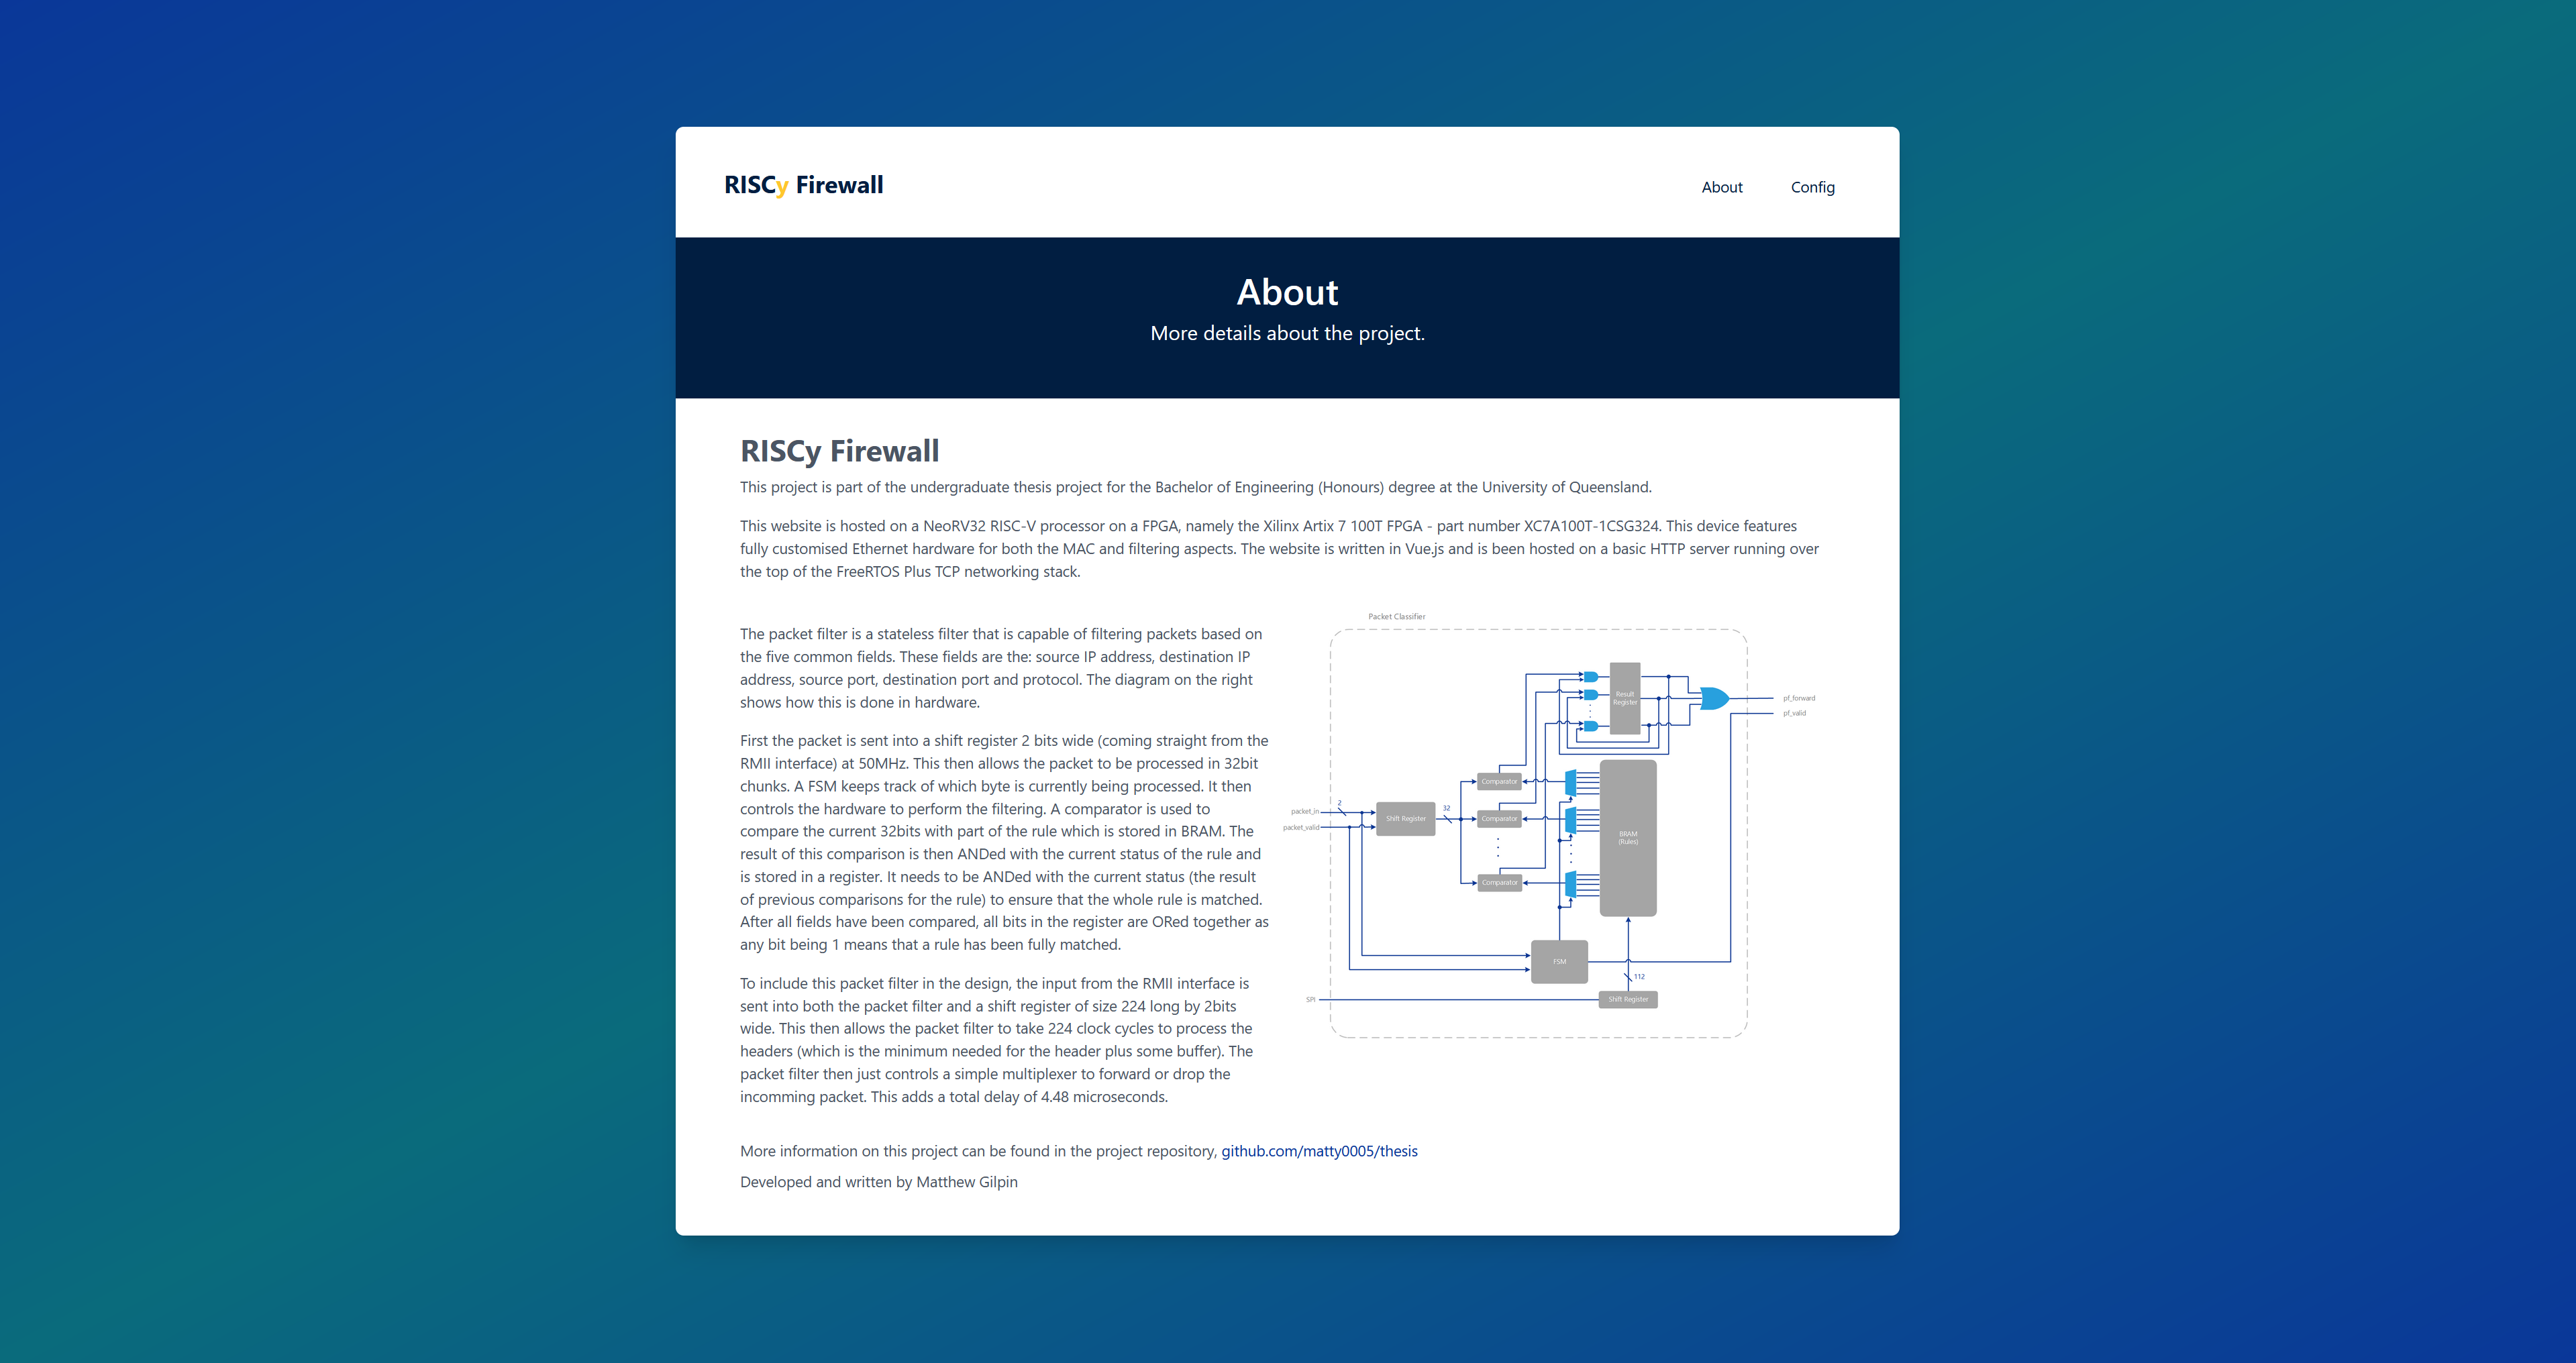
\includegraphics[width=1\textwidth]{Images/webapp_about.png}
    \caption{Screenshot of the about page in the webapp.}
    \label{fig:web_app_about}
\end{figure}

\begin{figure}[h!]
    \centering
    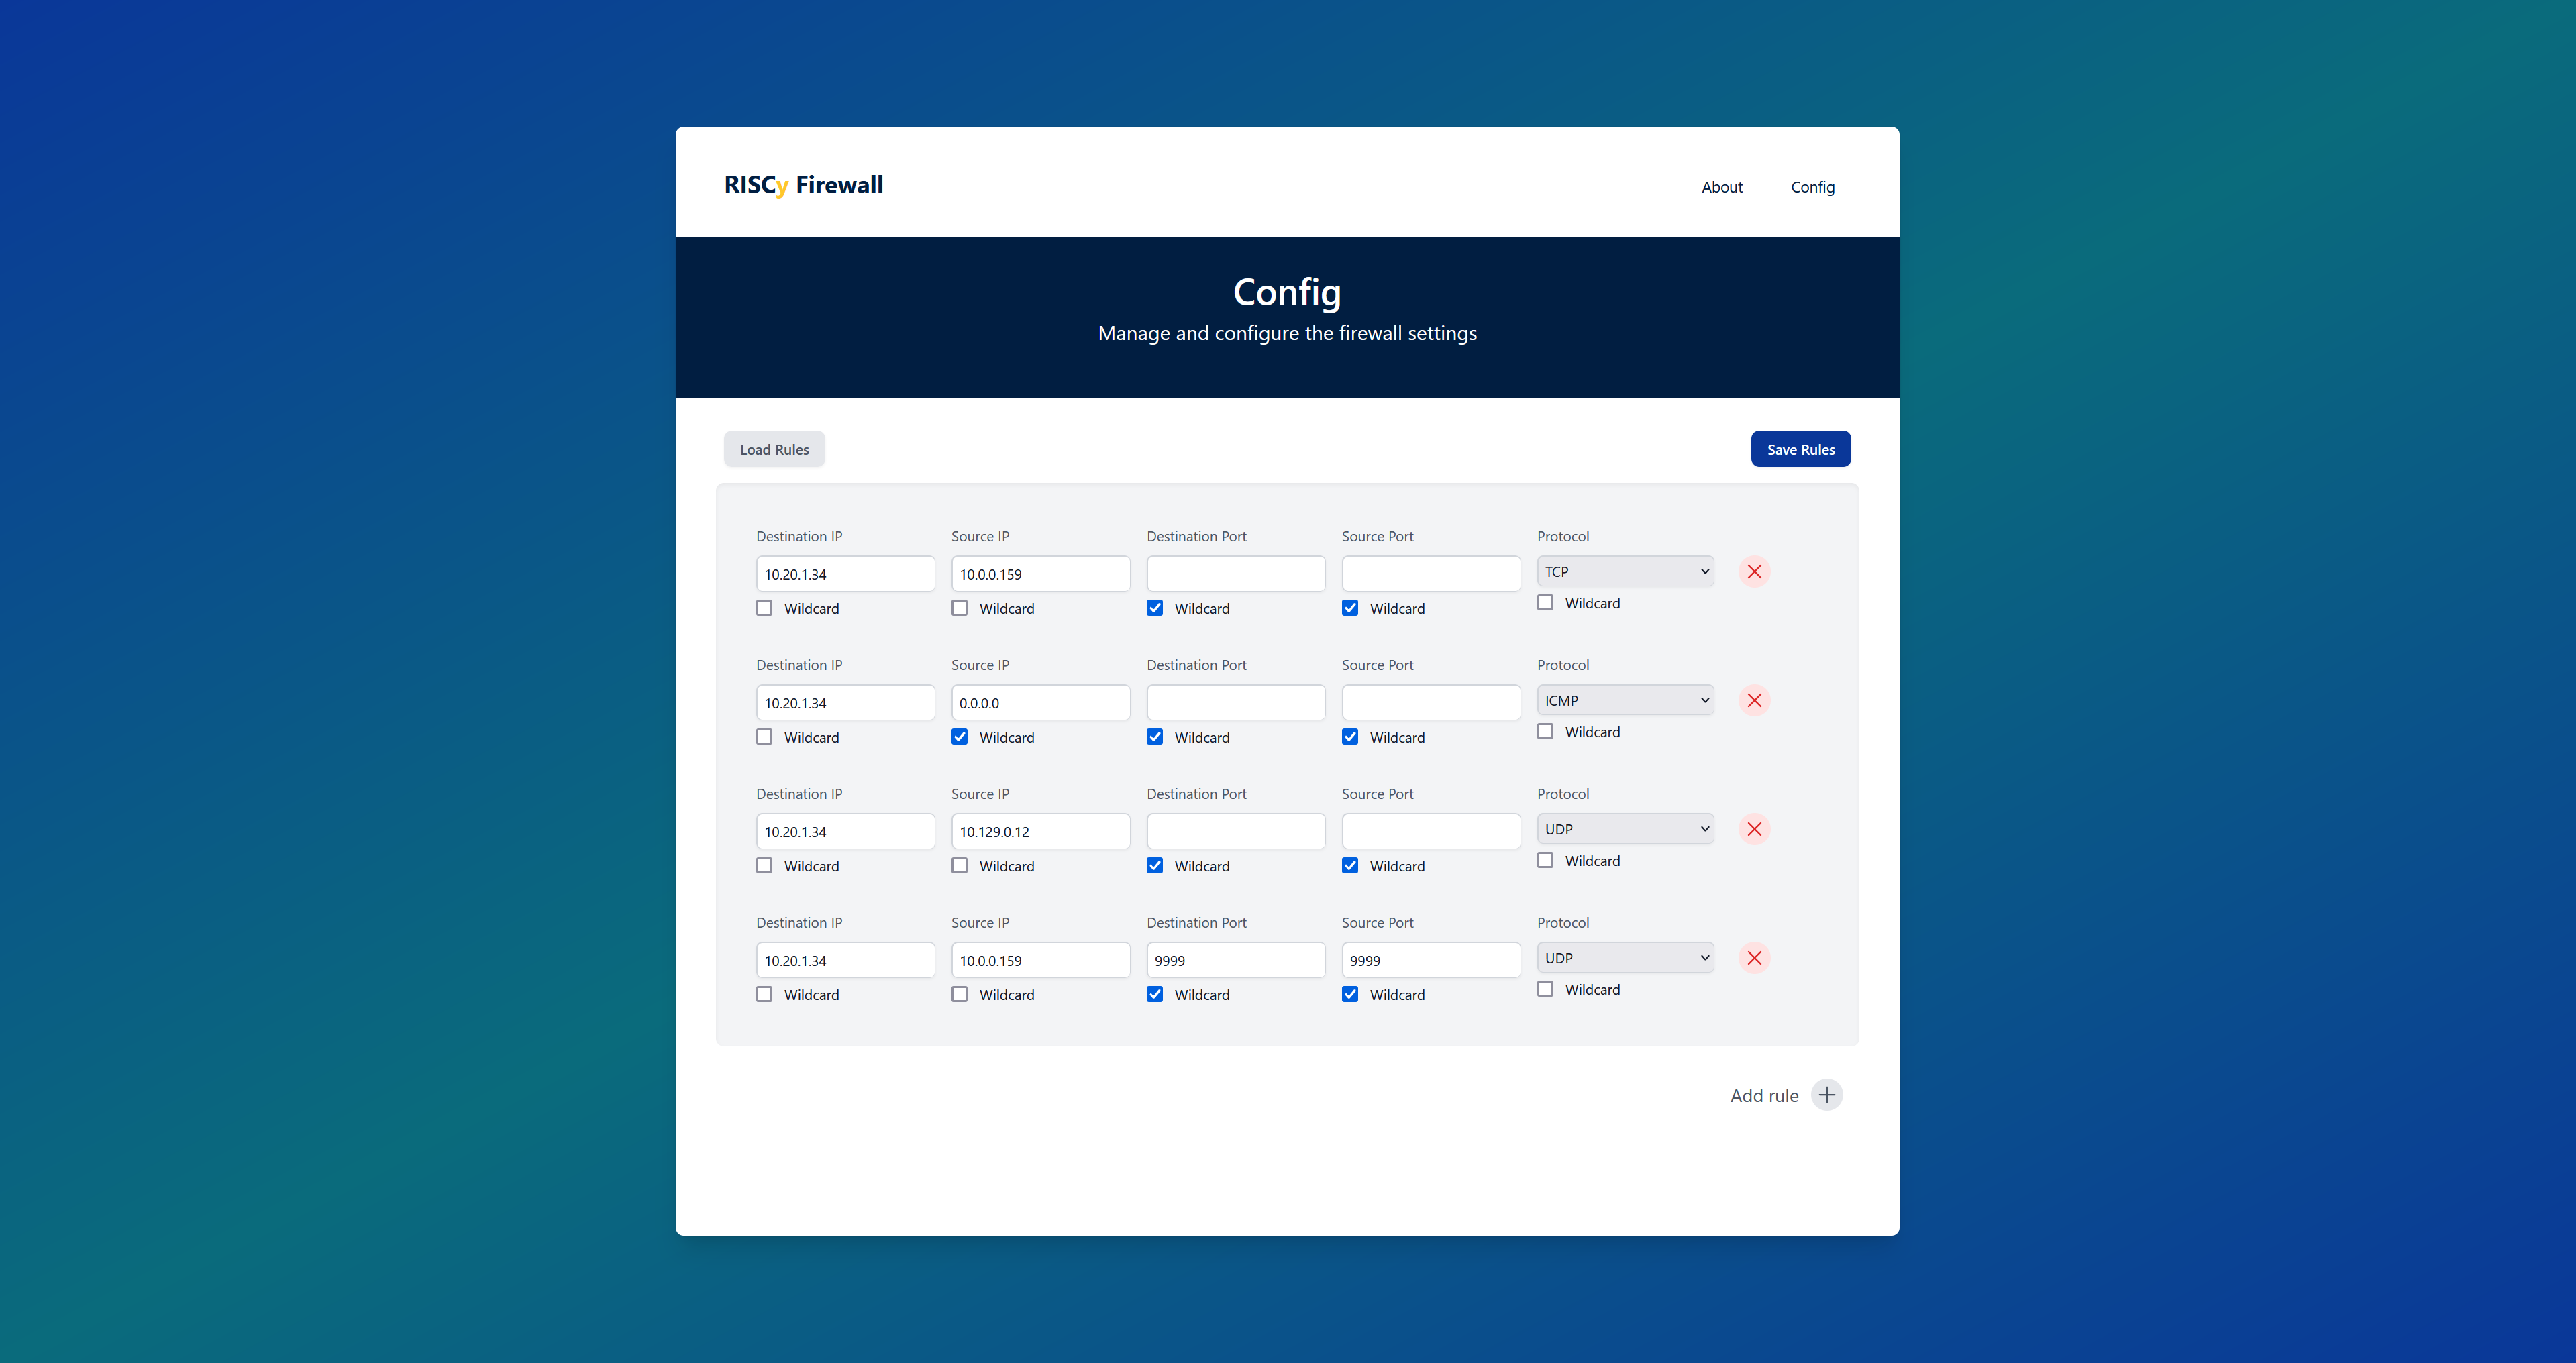
\includegraphics[width=1\textwidth]{Images/webapp_config.png}
    \caption{Screenshot of the config page in the webapp.}
    \label{fig:web_app_config}
\end{figure}


\section{UDP ping times between boards}
\label{app:udp_ping_measurements}
\begin{table}[ht]
    \centering
    \caption{Average UDP RTT for different devices and payload sizes.}
    \begin{tabular}{lcc}
    \toprule
    Device & 7 bytes (ms) & 256 bytes (ms) \\
    \midrule
    WIZ5500 Pico & 1.88 & 2.07 \\
    F767ZI & 1.30 & 1.39 \\
    F767ZI 80Mhz & 1.41 & 1.51 \\
    MilkV & 1.04 & 1.09 \\
    FPGA board & 1.45 & 1.72 \\
    \bottomrule
    \end{tabular}
    \end{table}

\section{Current measurments from boards}
\label{app:current_measurements}

Table \ref{tab:power_consumption} shows the current measurments. Notably Diff1 is the difference between the Idle and No ETH fields while Diff2 is the difference between the Idle and Clean states.

\begin{table}[ht]
    \centering
    \caption{Device power consumption data (all values in mA)}
    \label{tab:power_consumption}
    \begin{tabular}{lccccccc}
    \toprule
    Device    & Idle  & Busy  & Average  & No ETH  & Clean  & Diff1  & Diff2 \\
    \midrule
    FPGA      & 301.4     & 300.13    & 300.765      & 264         & 202.13           & 37.4     & 99.27       \\
    MilkV     & 76.27     & 76.53     & 76.4         & 69.23       & 69.23            & 7.04     & 7.04       \\
    F767ZI    & 209.25    & 206.9     & 208.075      & 153.46      & 121.31           & 55.79    & 87.94       \\
    WIZ5500   & 155.88    & 158.67    & 157.275      & 97.9        & 80.35            & 57.98    & 75.53       \\
    \bottomrule
    \end{tabular}
\end{table}


\section{Thermal measurements for boards}

\begin{table}[ht]
    \centering
    \caption{Device measurements over time using FLIR One thermal camera}
    \label{tab:measurements}
    \begin{tabular}{lcccccc}
    \toprule
    Device & 5min & 10min & 30min & 1h & 2h \\
    \midrule
    FPGA & 38 & 38.2 & 38.9 & 39.1 & 40.4 \\
    MilkV & 36.7 & 39.8 & 35.5 & 39.1 & 38.1 \\
    F767ZI (STM) & 35.9 & 38.9 & 35.8 & 37.5 & 36.8 \\
    F767ZI (PHY) & 38 & 38.8 & 35.2 & 37.2 & 36.2 \\
    WIZ5500 (RP2040) & 46.6 & 53.1 & 54.6 & 54.5 & 53.2 \\
    WIZ5500 (PHY) & 58 & 59 & 58.4 & 58.5 & 56.8 \\
    \bottomrule
\end{tabular}
\end{table}
